\chapter{Software di benchmark}
\fancyhead[RO]{\bfseries Software di benchmark}
\section{Definizione del software di benchmark}
Per valutare la qualità dell'algoritmo si è rivelato utile sviluppare un software in grado di raccogliere informazioni sull'efficenza dell'algoritmo stesso in tutte le possibili combinazioni di punto di arrivo/punto di partenza in mondi di dimensioni fissate. In particolare sono stati osservati i casi peggiori, la media aritmetica dei casi, lo scarto quadratico medio, e i risultati ottenuti più frequentemente. Il software permette di testare qualsiasi algoritmo in grado di interfacciarsi con il sistema di gioco. Non essendo presenti in letteratura algoritmi che risolvessero lo stesso problema qui trattato, ho ritenuto opportuno fare un confronto con un algoritmo greedy ottimo, che ha però bisogno di informazione completa sugli stati di ogni cella del mondo (anche senza aver fatto il movimento). Il termine di paragone è quindi il rapporto tra i valori raccolti attraverso l'esecuzione dell'algoritmo ottimo e quelli ottenuti con l'esecuzione dell'algoritmo descritto, più questo si avvicina ad 1, più le prestazioni dell'algoritmo sviluppato si avvicinano a quelle dell'algoritmo ottimo. Chiaramente il rapporto non sarà mai pari ad 1 a causa della differenza delle informazioni riguardo il mondo che i due agenti hanno, quindi la valutazione ha un carattere simbolico utilizzata in questo modo. Può però diventare interessante nel caso in cui vengano sviluppati altri algoritmi atti a risolvere la stessa problematica, per un confronto alla pari.

\section{Parametri che influenzano la qualità del risultato}
Ci sono dei parametri che possono essere modificati influenzando i risultati. Uno di questi è il numero di volte in cui il Drone debba passare su uno stesso punto prima di decidere di cambiare strategia e riniziare con la calibrazione. Attraverso l'osservazione dei diversi casi si è notato che facilmente l'agente può trovarsi a passare due volte nello stesso punto durante la ricerca (nel caso ad esempio si stia allontando dalla sorgente durante un movimento in diagonale), ma, date dimensioni del mondo relativamente grandi, è probabile che incorrendo tre o più volte nello stesso punto si stia entrando in un loop di movimenti, specialmente nel caso in cui la dimensione del grafo che rappresenta il KB  sia controllata, e quindi il numero di nodi memorizzati minore del numero di passi effettuati.
Un altro parametro che influenza l'efficenza dell'algoritmo è il numero di passi in orrizontale e in verticale da far svolgere al Drone durante la calibrazione. Infatti svolgendo un solo passo per direzione, nel caso in cui l'obiettivo si trovi su uno degli assi che incrociano il punto di partenza, l'agente si muoverà comunque in diagonale, per correggere in seguito la direzione, mentre permettendo di fare due passi in orizzontale, due in verticale e uno verso il punto di partenza in diagonale, nel caso in cui l'obiettivo si trovi su uno degli assi che si incontrano nell'ultimo punto in cui ci si è spostati, il drone andrebbe direttamente nella direzione del punto di arrivo. Si è notato però che questo approccio non modifica significativamente i risultati nel caso di dimensioni del mondo relativamente grandi, e ne peggiora la media nel caso di piccole dimensioni, quindi è stato preferito far svolgere all'agente un solo passo per direzione.
	
\section{Risultati}
I risultati dell'algoritmo cambiano anche qui in base ad altre condizioni: ad esempio nel caso in cui uno fra il Drone e il punto di arrivo si trovi ai bordi della matrice. Questo perchè, in questi casi, il problema è stato affrontato cercando una soluzione che permettesse semplicemente di evitare eventuali errori di esecuzione, falsando in qualche modo l'esecuzione dell'algoritmo, in quanto la tecnica è pensata per lavorare in campo aperto, in assenza di ostacoli. L'algoritmo arriva comunque a una soluzione, ma ha bisogno di più passaggi perchè appunto questa è una situazione anomala. E' stato quindi deciso di valutare la bontà dell'algoritmo escludendo queste situazioni, effettuando i test per tutte le posizioni possibili escluse quelle che portano sicuramente ad una situazione di eccezione. Tale situazione potrebbe incorrere anche in altri casi, ma questo è parte del problema (se il Drone si allontana dal punto di arrivo e va verso il bordo pur non essendo questo situato in posizioni estreme) e quindi ci si è limitati ad escludere le situazioni sfavorevoli a priori causate da problematiche tecniche e non intrinseche al problema.
Queste sono le schermate per testare l'algoritmo su una matrice 20x20:
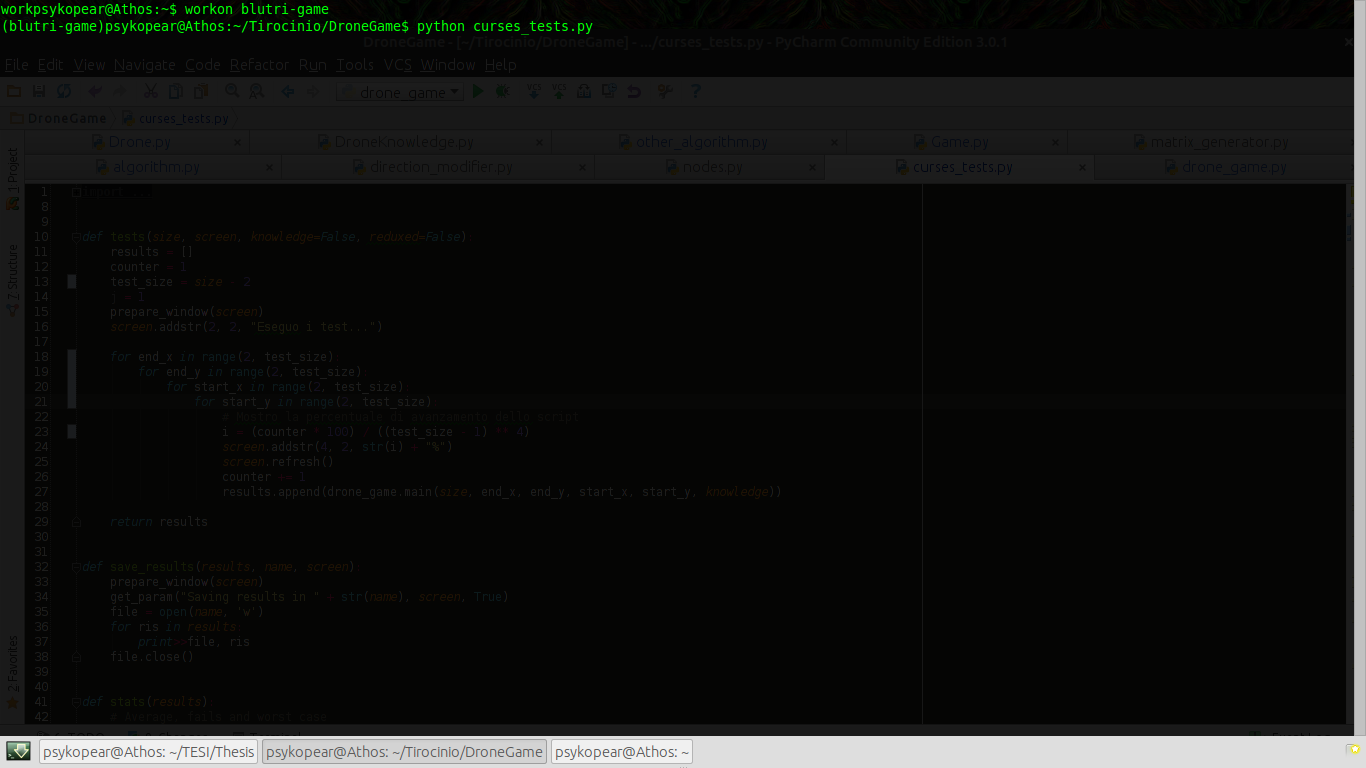
\includegraphics[width=\textwidth]{immagini/Test1.png}
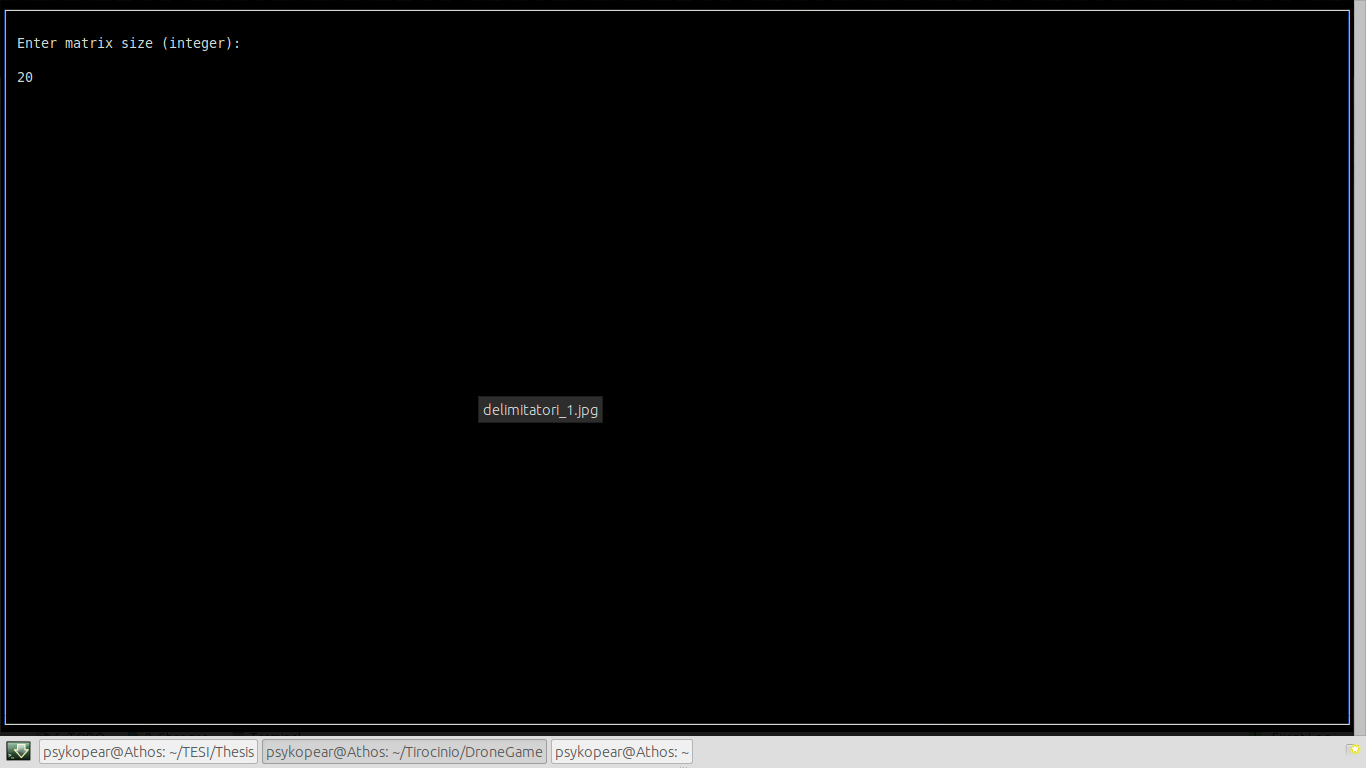
\includegraphics[width=\textwidth]{immagini/Test1-1.png}
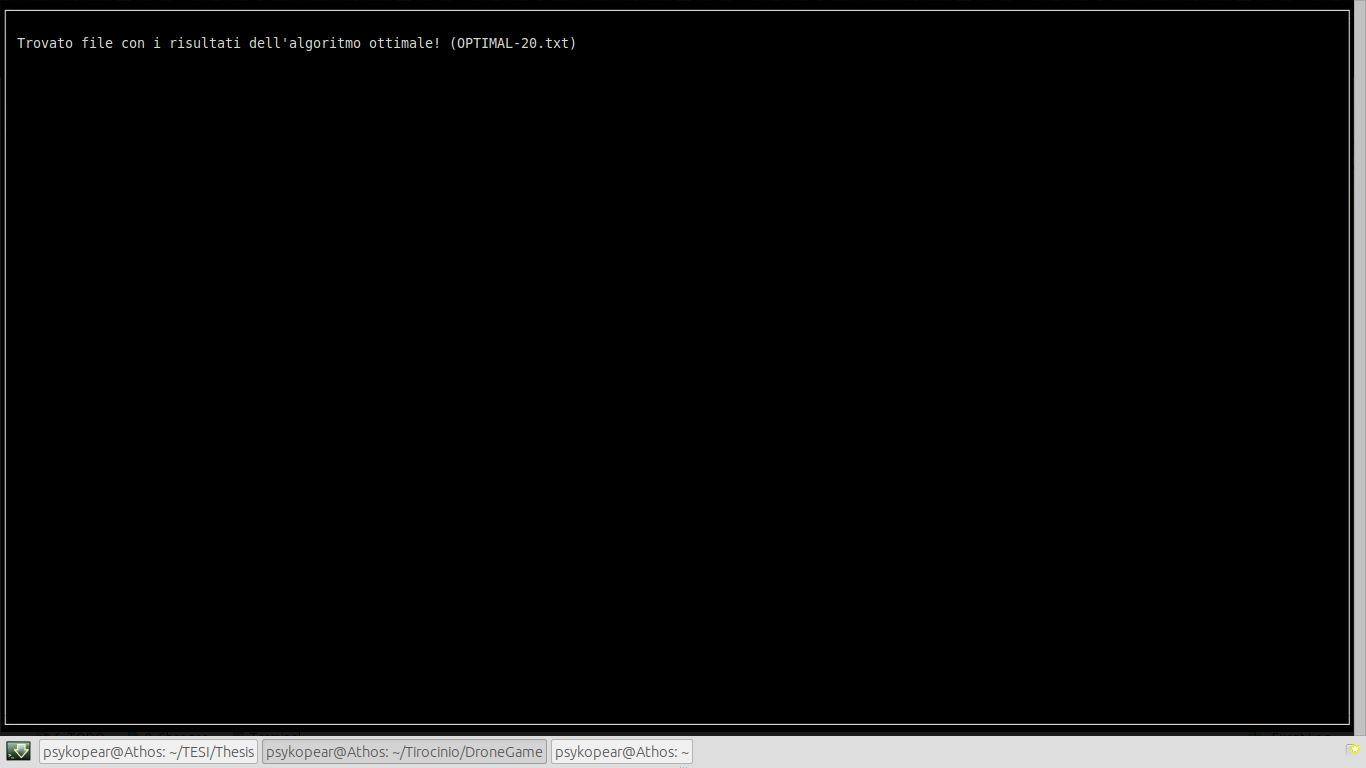
\includegraphics[width=\textwidth]{immagini/test2.png}
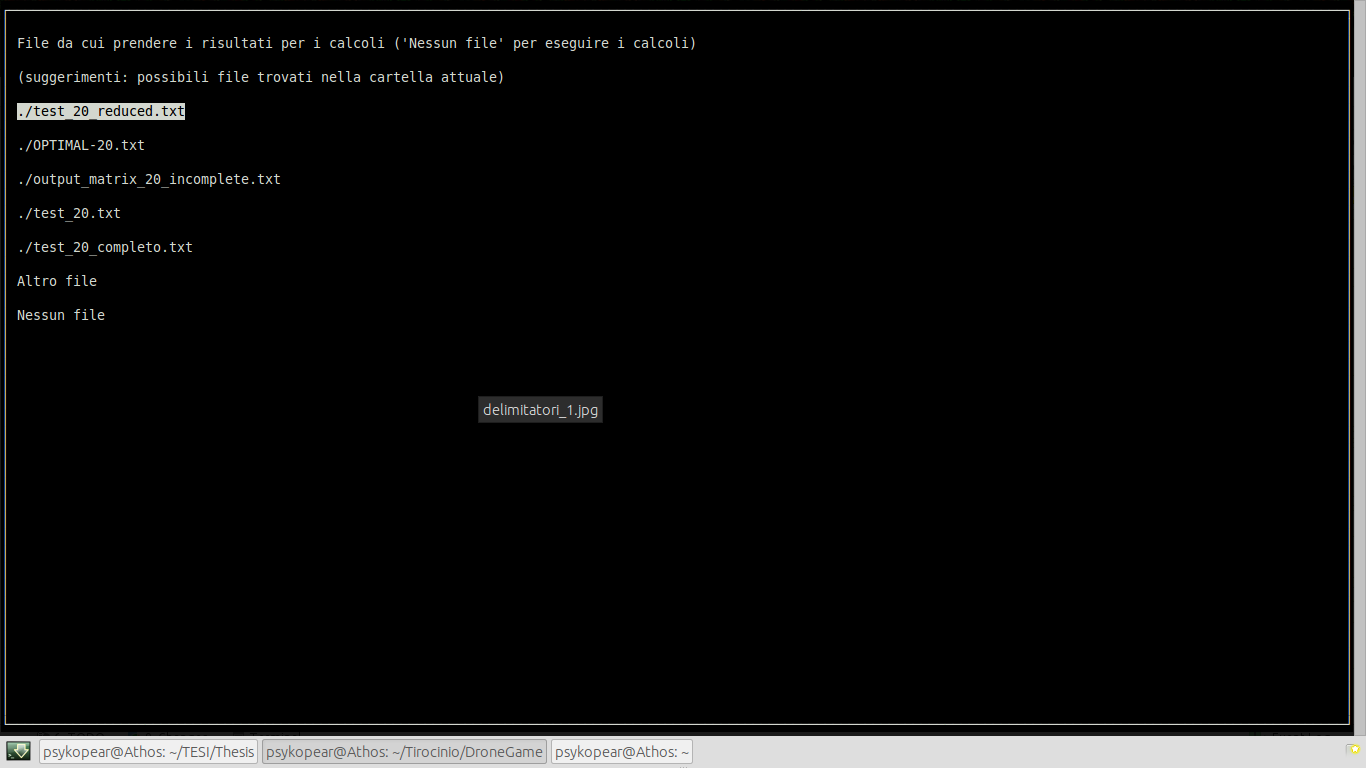
\includegraphics[width=\textwidth]{immagini/test3.png}
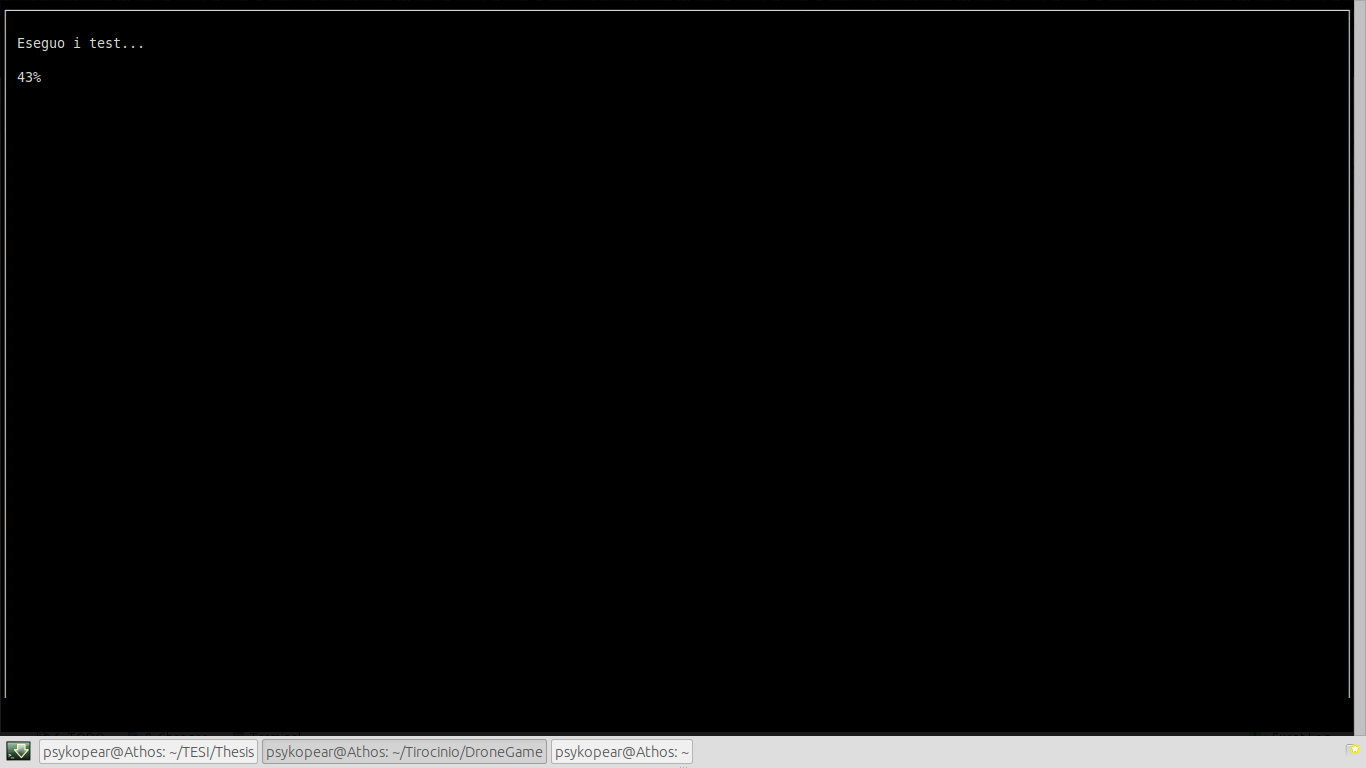
\includegraphics[width=\textwidth]{immagini/test5.png}
E questi sono i risultati ottenuti:\\*
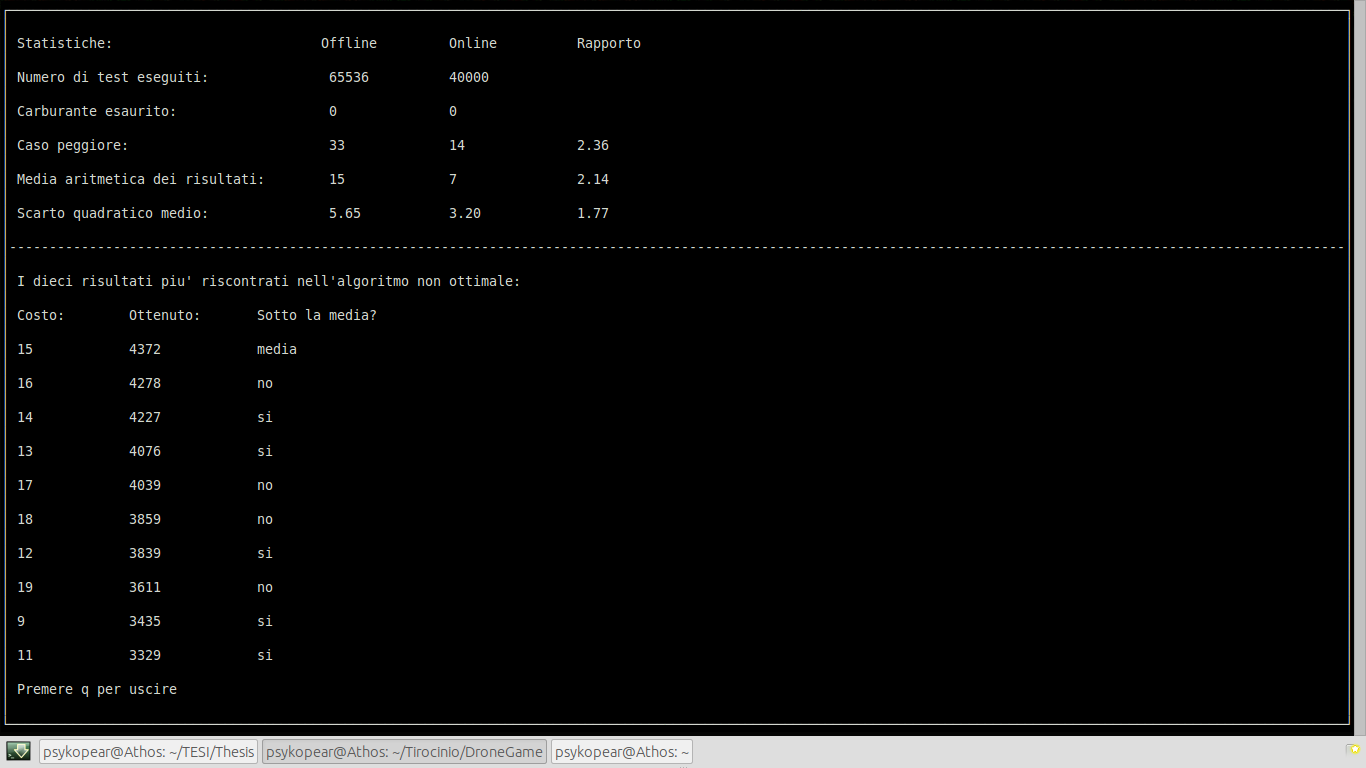
\includegraphics[width=\textwidth]{immagini/Results.png}